\section{Entregables y Sprits}
Como resultado final del desarrollo del proyecto se espera que éste concluya con un sistema web de la siguiente forma:
\begin{enumerate}
    \item Usuarios: Este módulo se encargará de la gestión de los candidatos, administradores y
    reclutadores
    \begin{enumerate}
        \item Candidatos: Estos podrán crear un perfil, realizar búsquedas y aplicar a vacantes.
        \item Reclutador: Estos podrán crear un perfil, publicar, modificar, eliminar vacantes y administrar el
        proceso de selección.
        \item Administrador: Este podrá consultar, dar de alta, modificar y eliminar a un reclutador y a colaboradores para 
        la gestión de la bolsa de trabajo.
    \end{enumerate}

    \item Administración de Solicitudes: En este módulo se implementará un mecanismo para la administración
    de las solicitudes.
    \item Módulo Currículum: En este módulo se implementará el generado automático de currículums y las
    sugerencias para el si es que las requiere.
    \item Administración y Filtro de Vacantes: Este módulo permite a los reclutadores gestionar las
    vacantes de la empresa a la que pertenece y a los candidatos consultarlas según sus aptitudes y habilidades.
\end{enumerate}

Los Sprits que se trabajarón durante TT-1 son:

\subsection{Sprint 1: Pruebas de concepto}
Esta iteración tuvo como propósito capacitarnos en las tecnologías que se van ha estar utilizando 
a lo largo del desarrollo del sistema.La actividades que se realizaron las siguientes:

\begin{enumerate}
    \item Crear el product backlog así como elementos de apoyo para dar prioridad y seguimiento.
    \item Especificar el lugar físico en el que el código del proyecto se va almacenar y que permita que
    todos los miembros del equipo puedan darle mantenimiento.
    \item Configurar las diferentes plataformas y tecnologías necesarias para el proyectot.
\end{enumerate}

\subsection{Sprint 2: Análisis y Planificación general del sistema Product Backlog}
Esta iteración tuvo como establecer los fundamentos teóricos y prácticos para su desarrollo.Las actividades que se realizaron 
de manera general fueron las siguientes:
\begin{enumerate}
    \item Implementar los requerimientos de prioridad alta.
    \item Diseñar e implementar las interfaces de usuario para la gestión de autenticación y gestión de
    participantes.
    \item Especificar los requerimientos mediante casos de uso y sus respectivas interfaces de usuario.
    \item Para este sprint se definieron los requerimientos funcionales para llevar a cabo los módulos
    correspondientes al desarrollo de esta iteración.
\end{enumerate} 

\subsection{Sprint 3: Gestión de Usuarios}
Esta iteración tuvo como propósito implementar un mecanismo que permita a
los usuarios del sistema autenticarse o crear cuentas para acceder al sistema, así como definir los
roles y los participantes del proyecto.


Los requerimientos funcionales de este sprint son:

\begin{longtable}{| p{0.15\textwidth}  | p{0.30\textwidth} | p{0.45\textwidth}  |}

    \label{table:herramientasSimilares}
        \rowcolor{black}
        %\multicolumn{7}{ |c| }{\bf\cellcolor{black}\color{white}{Herramientas para la especificación de requerimientos}} \\ \hline
        \bf\color{white} ID & \bf \color{white}Nombre	& \bf \color{white}Descripción \\ \hline
    \endhead
    RF-001 &Iniciar sesión & \\ \hline
    RF-002 &Crear cuenta & \\ \hline
    RF-003 &Enviar pre-registro & \\ \hline
    RF-004 &Configurar perfil & \\ \hline
    %\caption{Comparación Plataformas para buscar empleo}
\end{longtable}



\subsection{Sprint 4: Gestión de Vacantes}

Esta iteración tuvo como propósito implementar un mecanismo para gestionar las vacantes dentro del sistema.


Los requerimientos funcionales de este sprint son:
\begin{longtable}{| p{0.15\textwidth}  | p{0.30\textwidth} | p{0.45\textwidth}  |}

    \label{table:herramientasSimilares}
        \rowcolor{black}
        %\multicolumn{7}{ |c| }{\bf\cellcolor{black}\color{white}{Herramientas para la especificación de requerimientos}} \\ \hline
        \bf\color{white} ID & \bf \color{white}Nombre	& \bf \color{white}Descripción \\ \hline
    \endhead
    RF-006 &Publicar vacante& \\ \hline
    RF-011 &Consultar vacante & \\ \hline
    RF-012 &Listar vacante & \\ \hline
    %\caption{Comparación Plataformas para buscar empleo}
\end{longtable}

\subsection{Sprint 5: Gestión de Postulaciones}

Esta iteración tuvo como propósito implementar un mecanismo para gestionar las postulaciones dentro del sistema.


Los requerimientos funcionales de este sprint son:

\begin{longtable}{| p{0.15\textwidth}  | p{0.30\textwidth} | p{0.45\textwidth}  |}

    \label{table:herramientasSimilares}
        \rowcolor{black}
        %\multicolumn{7}{ |c| }{\bf\cellcolor{black}\color{white}{Herramientas para la especificación de requerimientos}} \\ \hline
        \bf\color{white} ID & \bf \color{white}Nombre	& \bf \color{white}Descripción
    \endhead
    RF-013 &Enviar Postulación& \\ \hline
    RF-016 &Listar Postulaciones & \\ \hline
    %\caption{Comparación Plataformas para buscar empleo}
\end{longtable}

\section{Casos de uso}


%\begin{UseCase}[]{USR-CU03.3}{ELiminar Idioma}{
	%Permite al alumno consultar la información de sus idiomas registrados en el perfil.
}
	%----------------------------------------------------------------
	% Datos generales del CU:
	\UCsection{Atributos}
	\UCitem{Actor(es)}{
		\Titem Candidato. 
	}
	\UCitem[admin]{Prioridad}{ 
		\Titem Media.
	}
	\UCitem[admin]{Complejidad}{
		\Titem Baja
	}
	\UCitem{Precondiciones}{
		\Titem El alumno debe de tener una cuenta en el sistema.
		\Titem Se debe de tener previmante registrado al menos un idioma.
	}
	\UCitem{Destino}{
		\Titem \refElem{USR-IU03.1}
	}
	\UCitem{Reglas de Negocio}{
		\Titem Ninguna.
		
	}
	\UCitem{Viene de}{
		\Titem Caso de uso \refIdElem{USR-CU03}.
	}	
\end{UseCase}

%Trayectoria Principal
\begin{UCtrayectoria}
	\UCpaso [\UCactor] Presiona el botón \IUEliminar{} desde la interfaz \refElem{USR-IU03}.
    \UCpaso [\UCsist] Muestra la interfaz \refElem{USR-IU03.3}.
	\UCpaso [\UCactor] Presiona el botón \IUbutton{Aceptar}.\refTray{A}
	\UCpaso [\UCsist] Agrega al catalogo de idiomas el idioma que se quiere eliminar.
	\UCpaso [\UCsist] Eliminar el registro del idioma en el sistem.
	\UCpaso [\UCsist] Muestra la información actualizada en la interfaz \refElem{USR-IU03}.
\end{UCtrayectoria}

\begin{UCtrayectoriaA}[Fin del caso de uso]{A}{El actor desea cancelar el registro}
	\UCpaso [\UCsist] Presiona el botón \IUbutton{Cancelar}.
	\extendUC{USR-CU03}.
\end{UCtrayectoriaA} 


%\begin{UseCase}[]{USR-CU03.3}{ELiminar Idioma}{
	%Permite al alumno consultar la información de sus idiomas registrados en el perfil.
}
	%----------------------------------------------------------------
	% Datos generales del CU:
	\UCsection{Atributos}
	\UCitem{Actor(es)}{
		\Titem Candidato. 
	}
	\UCitem[admin]{Prioridad}{ 
		\Titem Media.
	}
	\UCitem[admin]{Complejidad}{
		\Titem Baja
	}
	\UCitem{Precondiciones}{
		\Titem El alumno debe de tener una cuenta en el sistema.
		\Titem Se debe de tener previmante registrado al menos un idioma.
	}
	\UCitem{Destino}{
		\Titem \refElem{USR-IU03.1}
	}
	\UCitem{Reglas de Negocio}{
		\Titem Ninguna.
		
	}
	\UCitem{Viene de}{
		\Titem Caso de uso \refIdElem{USR-CU03}.
	}	
\end{UseCase}

%Trayectoria Principal
\begin{UCtrayectoria}
	\UCpaso [\UCactor] Presiona el botón \IUEliminar{} desde la interfaz \refElem{USR-IU03}.
    \UCpaso [\UCsist] Muestra la interfaz \refElem{USR-IU03.3}.
	\UCpaso [\UCactor] Presiona el botón \IUbutton{Aceptar}.\refTray{A}
	\UCpaso [\UCsist] Agrega al catalogo de idiomas el idioma que se quiere eliminar.
	\UCpaso [\UCsist] Eliminar el registro del idioma en el sistem.
	\UCpaso [\UCsist] Muestra la información actualizada en la interfaz \refElem{USR-IU03}.
\end{UCtrayectoria}

\begin{UCtrayectoriaA}[Fin del caso de uso]{A}{El actor desea cancelar el registro}
	\UCpaso [\UCsist] Presiona el botón \IUbutton{Cancelar}.
	\extendUC{USR-CU03}.
\end{UCtrayectoriaA} 


%\clearpage
\subsection{USR-IU02.2 Editar Medios de contacto y redes sociales}

\subsubsection{Objetivo}
En la figura \refElem{USR-IU02.2} se muestra la interfaz correspondiente con la funcionalidad descrita en las
trayectorias del caso de uso \refElem{USR-CU02.2} , la cual permite al actor editar sus medios de contacto como son: correos, teléfonos y redes sociales.

\subsubsection{Comandos}
Los siguientes comandos aparecen en la interfaz descrita anteriormente.
\Titem \IUbutton{Aceptar} : Cuando presiona el botón, actualiza la información .
\Titem \IUbutton{Cancelar} : Cuando presiona el botón, muestra la sección anterior.%\refElem{GRL-IU02-2}.

\IUfig{.9}{CasosdeUso/USR-CU02-2/imagenes/USR-IU02.2.png}{USR-IU02.2}{Editar Medios de contacto y redes sociales}  


\clearpage


Los casos de uso son una herramienta usada para representar las transacciones entre un actor y el sistema, las cuales siempre tendrán un valor agregado o un propósito para que el actor las realice.
En estos se representan a traves de diagramas los cuales se conforan por los siguientes elementos:

\begin{itemize}
	 \UCpaso Representa al sistema mediante un óvalo.
	\item \UCactor Representa al actor que va a interactuar con el sistema.
	\item Relación $<$- - -$<<extends>>$- - -. Indica que un caso de uso \textbf{puede} ejecutarse a partir de otro.
	\item Relación - - -$<<include>>$- - -$>$. Indica que un caso de uso \textbf{debe} ejecutarse a partir de otro.
\end{itemize}

La conexión entre un actor y un caso de uso es por medio de una línea como se muestra en la figura \ref{fig:acUC}.

\begin{figure}[hbtp!]
	\begin{center}
		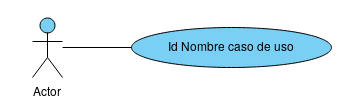
\includegraphics[width=.4\textwidth]{LIT/ActorUC}
	\end{center}
	\label{fig:acUC}
	\caption{Interacción del actor con el caso de uso}
\end{figure}

Los casos de uso se encontrarán dentro de paquetes (representados por carpetas) indicando así que pertenecen a un mismo módulo como se muestra en la figura \ref{fig:pack}.

\begin{figure}[hbtp!]
	\begin{center}
		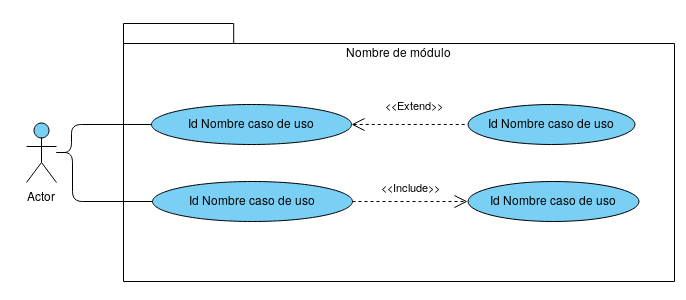
\includegraphics[width=.7\textwidth]{LIT/Paquete}
	\end{center}
	\label{fig:pack}
	\caption{Un Actor con varios caso de uso dentro de un módulo}
\end{figure}

\pagebreak

\subsection{Identificadores de casos de uso}

Los casos de uso se identificarán de acuerdo a la siguiente nomenclatura:

\begin{figure}[hbtp!]
	\begin{center}
		
\includegraphics[width=.7\textwidth]{LIT/UCnombre}
	\end{center}
	\label{fig:nomenclatura}
\end{figure}

%\subsection{Modelado de Máquinas de Estados}
  %      \label{sec:ModMaquinas}

%\subsection{Modelado de Actores}
 %       \label{sec:ModActores}
%- - - - - - - - - - - - - - - - - - - - - - - - - - - - -
\subsection{Especificación de casos de uso}

Para poder entender un caso de uso más allá de un diagrama, se lleva a cabo la tarea de especificar cada uno de los casos de uso identificados en el sistema con el fin de describir las secuencias de acciones que realiza el sistema y que lleva a un resultado de valor a un actor específico. Los casos de uso tienen atributos los cuales se describen a continuación:

\begin{description}
	\item[Id] Identificador del caso de uso, el cual debe ser único.
	\item[Nombre] Nombre del caso de uso el cual es descriptivo basándose en la transacción que se realiza.
	\item[Resumen] Es una descripción resumida en la que se especifica la transacción realizada por el caso de uso.
	\item[Actores] Lista de los actores que interactúan con el caso de uso.
	\item[Entradas] Lista los datos de entrada que el caso de uso recibe, los cuales harán referencia al modelo de información.
	\item[Salidas] Lista los datos de salida que el caso de uso genera, por ejemplo: 
	\item[Destino] Indica a dónde se dirigen los datos de salida, por ejemplo: pantalla, impresora, repositorio, hacia un servidor o un archivo.
	\item[Precondiciones] Enlista las cosas que deben haber sucedido para que el caso  de uso se lleve a cabo.
	\item[Postcondiciones] Enlista las cosas que suceden en el sistema o negocio de forma inmediata o a corto plazo una vez que se ejecute el caso de uso.
	\item[Reglas de Negocio] Lista las reglas de negocio que se van a ejecutar en el caso de uso.
	\item[Viene de] Indica cuando el caso de uso se extiende de otro o se incluye en otro.
	\item[Trayectoria principal] Secuencia de pasos que llevan al caso de uso al éxito.
	\item[Trayectoria(s) alternativa(s)] Secuencias de pasos que llevan al caso de uso al éxito o al fracaso.
	\item[Puntos de extensión] Cuando existen casos de uso que pueden ejecutarse a partir del caso de uso en proceso.
\end{description}


%---------------------------------------------------------
\subsection{Modelado de casos de uso}

\subsubsection{Modelo de estados}

Diversas entidades en el sistema  que tienen un comportamiento dinámico en el sistema, 
los que se consideraron en el desarrollo del sistema y ameritaban ser modelados a través de una 
maquina de estados.\\

\subsubsection{Actores del sistema}
 Se definen los actores identificados como participantes en los procesos del sistema. 
 Estos actores son los encargados de llevar a cabo determinadas tareas dentro de cada proceso.\\
 
 \subsubsection{Reglas de negocio}

 Se van describir las reglas de negocio identificadas en el sistema las cuales son una condición que 
 se debe satisfacer cuando se realiza una actividad de negocio.\\
 
\subsubsection{Casos de uso}

Las funcionalidades del sistema son representadas mediante casos de uso. Un caso de uso es una transacción entre un actor y el sistema que tiene un valor agregado o un propósito para que el actor las realice. Los casos de uso se modelan a partir de dos elementos: un diagrama de casos de uso y la
descripción del caso de uso.\\

\subsubsection{Mensajes del sistema}

Los mensajes se refieren a todos aquellos avisos que el sistema muestra al actor para comunicar la ocurrencia de algún evento tal como un error o una operación exitosa. 


